\documentclass[main.tex]{subfiles}
\begin{document}

\chapter{Talen en Automaten}
\label{cha:talen-en-automaten}

\section{Symbolen en Strings}
\label{sec:symbolen-en-strings}

\begin{de}
  Een \term{symbool} $s$ is een representatie van een object in de abstractste zin van het woord. 
\end{de}

\begin{de}
  Een alfabet $\Sigma$ is een eindige verzameling van symbolen.
\end{de}

\begin{de}
  Een \term{string} $s$ over een alfabet $\Sigma$ is een geordende opeenvolging van nul, \'e\'en of meer elementen van $\Sigma$. Symbolen zijn dus strings van lengte 1.
  \[ s = a_{1}\ldots a_{n} \text{ met } a_{i} \in \Sigma \]
\end{de}

\begin{de}
  $\epsilon$ is de \term{string} zonder symbolen en noemen we de \term{lege string}.
\end{de}

\begin{opm}
  Bij twijfel kan elk symbool gezien worden als een string van lengte $1$.
\end{opm}

\begin{de}
  De \term{concatenatie} $xy$ van twee strings $x = \{x_1,x_2,\ldots,x_m\}$ en $y =   \{y_1,y_2,\ldots,y_n\}$ is de volgende geordende verzameling  
  \[
  xy = \{ x_1,x_2,\ldots,x_m,y_1,y_2,\ldots,y_n\}
  \] 
\end{de}

\begin{ei}
  De concatenatie van strings is associatief:
  \[
  (xy)z = x(yz)
  \]

  \begin{proof}
    \[
    \begin{array}{r l l}
      (xy)z &= \{x_1,x_2,\ldots,x_m,y_1,y_2,\ldots,y_n\}z &\\
            &= \{x_1,x_2,\ldots,x_m,y_1,y_2,\ldots,y_n,z_1,z_2,\ldots,z_o\} &\\
            &= x\{y_1,y_2,\ldots,y_n,z_1,z_2,\ldots,z_o\} &= x(yz)
    \end{array}
    \]
  \end{proof}
\end{ei}

\begin{de} 
  De verzameling van alle eindige strings over een alfabet $\Sigma$ noteren we als $\Sigma^{*}$.
  \[ \Sigma^{*} = \{ a_{1}a_{2}\ldots a_{n}\ |\ a_{i}\in \Sigma,\ n,i\in \mathbb{N} \} \]
\end{de}

\begin{de}
  De verzameling $\Sigma \cup \{\epsilon\}$ noteren we korter als $\Sigma_{\epsilon}$.
  Merk op dat dit niet zomaar een verzameling symbolen is. $\epsilon$ is namelijk een string.
\end{de}

\begin{de}
  De \term{omgekeerde string} $s^{R}$ van een string $s$ is de string waarbij de symbolen van $s$ in omgekeerde volgorde staan.
  \[ s = a_{n}\ldots a_{1} \text{ met } a_{i} \in \Sigma \]
\end{de}

\section{Talen}
\label{sec:talen}

\begin{de}
  Een \term{taal} $L$ over een alfabet $\Sigma$ is een verzameling van eindige strings over $\Sigma$.
\end{de}

\begin{de}
  De \term{concatenatie} $L_1L_2$ \term{van twee talen} $L_1$ en $L_2$ over hetzelfde alfabet $\Sigma$ is de volgende verzameling:
  \[
  L_1L_2 = \{\ xy\ |\ x \in L_1,\ y \in L_2\ \} 
  \]
\end{de}

\begin{ei}
  De concatenatie van talen is associatief:
  \[
  (L_1L_2)L_3 = L_1(L_2L_3)
  \]

  \begin{proof}
    \[
    \begin{array}{r l l}
      (L_1L_2)L_3 &= \{\ xy\ |\ x \in L_1,\ y \in L_2\ \}L_3 &\\
                 &= \{\ xyz\ |\ x \in L_1,\ y \in L_2\,\ z \in L_3\} &\\
                 &= L_1\{\ yz\ |\ y \in L_2,\ z \in L_3\ \} &= L_1(L_2L_3)
    \end{array}
    \]
  \end{proof}
\end{ei}

\begin{ei}
  Talen, uitgerust met de unie, de doorsnede, het complement en de concatenatie, vormen een algebra.
  \begin{proof}
    Inderdaad, zowel de unie, de doorsnede, het complement als de concatenatie zijn inwendig. 
  \end{proof}
\end{ei}

\begin{de}
  De concatenatie van $n$ keer een taal $L$ met zichzelf noteren we als $L^n$.
  $L^0$ bevat enkel de lege string.
  \[
  L^0 = \{\epsilon\},\quad L^{n} = LL^{n-1}
  \]
\end{de}

\begin{de}
  De \term{Kleene-ster} $L^*$ van een taal $L$ is de unie van alle concatenaties van $L$ met zichzelf.
  \[
  L^* = \bigcup_{n=0}^{\infty}L^n
  \]
\end{de}

\begin{de}
  $L^{+}$ is de unie van $L$, \'e\'en of meer keer geconcateneerd met zichzelf.
  \[
  L^{+} = LL^{*}
  \]
\end{de}

\begin{ei}
  \label{ei:taal-alternatieve-definitie}
  We kunnen een taal ook defini\"eren als een deelverzameling van $\Sigma^{*}$ (of als een element van $\mathcal{P}(\Sigma^{*})$.)

  \begin{proof}
    Inderdaad, elke verzameling van eindige strings is een deelverzameling van de verzameling van alle eindige strings, alsook een element van de verzameling van alle deelverzamelingen van de verzameling van alle eindige strings.
  \end{proof}
\end{ei}

\begin{de}
  $L_{\Sigma}$ is de notatie voor de verzameling van alle \term{talen over een alfabet} $\Sigma$. 
  \[ L_{\Sigma} = \mathcal{P}(\Sigma^{*}) \]
\end{de}

\section{Reguliere expressies en talen}
\label{sec:reguliere-expressies-en-talen}

\begin{de}
  Een \term{reguliere expressie} (RE) wordt inductief gedefinieerd als een expressie van de volgende vorm:
  \begin{itemize}
  \item $\epsilon$
  \item $\phi$
  \item $a$ met $a \in \Sigma$
  \item $(E_1E_2)$ waarbij $E_1$ en $E_2$ reguliere expressies zijn over $\Sigma$
  \item $(E)^*$ waarbij $E$ een reguliere expressie is over $\Sigma$
  \item $(E_1|E_2)$ waarbij $E_1$ en $E_2$ reguliere expressies zijn over $\Sigma$
  \end{itemize}
  Merk op dat, net als strings, reguliere expressies steeds eindig zijn.
  Deze definitie laat immers geen oneindige reguliere expressies toe.
\end{de}

\begin{de}
  De verzameling van alle reguliere expressies over een alfabet $\Sigma$ noteren we als $RegEx_{\Sigma}$ of $RegEx$.
\end{de}

\begin{st}
  De verzameling van alle reguliere expressies $RegEx$ over een alfabet $\Sigma$ vormt een taal.

  \begin{proof}
    Inderdaad, voeg aan $\Sigma$ nog de volgende symbolen toe om $\Sigma'$ te bekomen: $\epsilon$, $\phi$, $($, $)$, $|$ en $^{*}$.
    Nu vormt de verzameling van alle reguliere expressies een taal over $\Sigma'$.

    Merk op dat deze taal \emph{niet} regulier\footnote{Zie de definitie van reguliere talen (Definitie \ref{de:reguliere-taal}).} is. Er zitten immers haakjes in die moeten samen passen. (Zie verder waarom dit dan geen reguliere taal is (TODO)) 
    \TODO{ voeg verwijzing toe zodra bewezen is dat $0^{n}1^{n}$ niet regulier is. }
  \end{proof}
\end{st}

\begin{de}
  \label{def:taal-bepaald-door-regex}
  De \term{taal bepaald door een reguliere expressie} $L_E$ over hetzelfde alfabet $\Sigma$ is de volgende.
  \[
  \begin{array}{|c|c|}
    \hline
    E                           & L_E\\
    \hline
    a \text{ met } a \in \Sigma & \{a\}\\
    \epsilon                    & {\epsilon}\\
    \phi                        & \emptyset\\
    (E_1E_2)                    & L_{E1}L_{E2}\\
    (E)^{*}                      & L_E^*\\
    (E_1|E_2)                   & L_{E1} \cup L_{E2}\\
    \hline
  \end{array}
  \]
\end{de}

\begin{de}
  \label{de:reguliere-taal}
  Een \term{reguliere taal} is een taal die bepaald wordt door een reguliere expressie.
\end{de}

\begin{ei}
  \label{ei:reguliere-taal-expressie}
  Voor elke reguliere taal bestaat er een reguliere expressie die die taal bepaalt.

  \begin{proof}
    Inderdaad, anders was het geen reguliere taal! \footnote{Zie de definitie van een reguliere taal (Definitie \ref{de:reguliere-taal}).}
  \end{proof}
\end{ei}

\begin{st}
  Als een reguliere expressie $E$ geen ster bevat, dan is de taal $L_{E}$ bepaald door die reguliere expressie eindig.
  
  \begin{proof}
    We tonen eerst de kardinaliteit van van $L_{E}$ afhankelijk van $E$.
    \[
    \begin{array}{|c|c|}
      \hline
      E                           & |L_E|\\
      \hline
      a \text{ met } a \in \Sigma & 1\\
      \epsilon                    & 1\\
      \phi                        & 0\\
      (E_1E_2)                    & |L_{E1}| \cdot |L_{E2}|\\
      (E)^{*}                      & \infty\\
      (E_1|E_2)                   & |L_{E1}| + |L_{E2}| - |L_{E1} \cap L_{E2}|\\
      \hline
    \end{array}
    \]
    Zoals we zien in de tabel blijft de kardinaliteit $L_{E}$ eindig zolang we geen ster gebruiken in $E$.
  \end{proof}
\end{st}

\begin{st}
  Als een reguliere expressie $E$ een ster bevat, is $L_{E}$ oneindig.
  \begin{proof}
    Inderdaad, als we opnieuw kijken naar de tabel met kardinaliteiten, zien we dat een ster in $E$ een oneindige kardinaliteit geeft voor $|L_{E}|$.
    Bovendien is er geen manier om een oneindige kardinaliteit in een reguliere expressie weg te werken door samenstelling van reguliere expressies.
    De kardinaliteit kan enkel oneindig blijven eens er een ster is gebruikt.
    $L_{E}$ is dus inderdaad oneindig zodra $E$ een ster bevat.
  \end{proof}
\end{st}

\begin{st}
  Zij $E$ en $F$ reguliere expressies. Nu geldt volgende bewering.
  \[ L_{E} \subseteq L_{(E|F)} \]

  \begin{proof}
    \[ L_{(E|F)} = L_{E} \cup L_{F}\]
    \[ L_{E} \subseteq L_{E} \cup L_{F} \]
  \end{proof}
\end{st}

\begin{de}
  $RegLan$ is \term{verzameling van alle reguliere talen}.
\end{de}

\begin{ei}
  $Reglan$ is een subalgebra van $L_{\Sigma}$.

  \begin{proof}
    Bewijs in delen.
    \begin{itemize}
    \item $RegLan$ is een deelverzameling van $L_{\Sigma}$.
      \[ RegLan \subseteq L_{\Sigma} \]
    \item De unie is inwendig in $RegLan$.\\
      Kies twee willekeurige reguliere talen $L_{E1},\ L_{E2} \in RegLan$.
      De unie $L_{E1} \cup L_{E2}$ van deze twee talen wordt bepaald door de reguliere expressie $(E_1|E_2)$ en is bijgevolg een reguliere taal.
      \footnote{Zie de definitie van de taal bepaald door een reguliere expressie. (Definite \ref{def:taal-bepaald-door-regex})}
    \item De concatenatie is inwendig in $RegLan$.\\
      Kies twee willekeurige reguliere talen $L_{E1},\ L_{E2} \in RegLan$.
      De concatenatie $L_{E1}L_{E2}$ van deze twee talen wordt bepaald door de reguliere expressie $E_1E_2$ en is bijgevolg een reguliere taal.
      \footnote{Zie de definitie van de taal bepaald door een reguliere expressie. (Definite \ref{def:taal-bepaald-door-regex})}
    \item Het complement is inwendig in $RegLan$.
      \TODO{Verwijzing naar bewijs (later)}
    \item De doorsnede is inwendig in $RegLan$.
      \TODO{Verwijzing naar bewijs (later)}
    \end{itemize}
  \end{proof}
\end{ei}

\begin{ei}
  Hier volgen een aantal eigenschappen over $RegLan$.
  \begin{enumerate}
  \item $RegLan \subseteq \Sigma$: Onwaar, er wordt hier een verzameling talen met een verzameling symbolen vergeleken.
  \item $RegLan \subseteq \Sigma^{*}$: Onwaar, er wordt hier een verzameling talen met een verzameling strings vergeleken.
  \item $RegLan \subseteq \mathcal P(\Sigma)$: Onwaar, er wordt hier een verzameling talen met een verzameling van verzamelingen van symbolen vergeleken.
  \item $RegLan \subseteq \mathcal P(\Sigma^{*})$: Waar, dit is equivalent met: ``Een reguliere taal is een taal.''.
  \item $RegLan \subseteq \mathcal P(\mathcal P(\Sigma^{*}))$: Onwaar, er wordt hier een verzameling talen vergeleken met een een verzameling van verzamelingen van talen. Merk op dat, als er '$\in$' stond in plaats van '$\subseteq$', deze stelling wel klopte.
  \item $(\forall x)(x \in RegLan \Rightarrow x \in \Sigma)$: Onwaar, zie puntje 1.
  \item $(\forall x)(x \in RegLan \Rightarrow x \in \Sigma^{*})$: Onwaar, zie puntje 2.
  \item $(\forall x)(x \in RegLan \Rightarrow x \in \mathcal P(\Sigma))$: Onwaar, zie puntje 3.
  \item $(\forall x)(x \in RegLan \Rightarrow x \in \mathcal P(\Sigma^{*}))$: Waar, zie puntje 4.
  \item $(\forall x)(x \in RegLan \Rightarrow x \in \mathcal P(\mathcal P(\Sigma^{*})))$: Onwaar, zie puntje 5.
  \item $(\forall x,y)(x \in RegLan \wedge y \in x \Rightarrow y \in \Sigma)$: Onwaar, $y$ is hier een string terwijl $x$ een taal is. De uitdrukking $y \in \Sigma$ is dus triviaal fout.
  \item $(\forall x,y)(x \in RegLan \wedge y \in x \Rightarrow y \in \Sigma^{*})$: Waar, dit is equivalent met: ``Een string van een reguliere taal is een string.''.
  \item $(\forall x,y)(x \in RegLan \wedge y \in x \Rightarrow y \in \mathcal P(\Sigma)$: Onwaar, $y$ is een string, maar $\mathcal P(\Sigma)$ is een verzameling van verzamelingen symbolen. Er is op deze twee geen 'element van' gedefinieerd.
  \item $(\forall x,y)(x \in RegLan \wedge y \in x \Rightarrow y \in \mathcal P(\Sigma^{*})$: Onwaar, $y$ is een string, maar $\mathcal P(\Sigma^{*})$ is een verzameling talen. Er is op deze twee geen 'element van' gedefinieerd.
  \item $(\forall x,y)(x \in RegLan \wedge y \in x \Rightarrow y \in \mathcal P(\mathcal P(\Sigma^{*}))$: Onwaar, $y$ is een string, maar $\mathcal P(\mathcal P(\Sigma^{*}))$ is een verzameling van verzamelingen van talen. Er is op deze twee geen 'element van' gedefinieerd.
  \end{enumerate}
\end{ei}

\begin{st}
  Er bestaat een niet-reguliere taal.

  \begin{proof}
    Elke reguliere expressie bepaalt precies \'e\'en (reguliere) taal.
    Er zijn aftelbaar oneindig veel reguliere expressies en bijgevolg hoogstens aftelbaar oneindig veel reguliere talen.
    Er zijn echter overaftelbaar oneindig veel talen. Er moet dus minstens \'e\'en niet-reguliere taal bestaan.
    (In feite zijn de meeste\footnote{'de meeste' heeft een heel specifieke wiskundige betekenis.} talen niet-regulier.)
  \end{proof}
\end{st}

\begin{st}
  Elke eindige taal $L$ is regulier.

  \begin{proof}
    We bewijzen dit door de constructie van een reguliere expressie die $L$ bepaalt:\\
    Zij $n$ het aantal strings in $L$ met $n$ eindig.
    Voor elke string $s_{i} \in L$, construeren we een reguliere expressie $E_{i}$ die de taal met enkel $s_{i}$ bepaalt door de concatenatie van de opeenvolgende symbolen in $s_{i}$. 
    Voeg nu al deze reguliere expressies $E_{i}$ samen tot $(E_{1}|E_{2}|\ldots|E_{n})$ om de reguliere expressie te krijgen die $L$ bepaalt.
  \end{proof}
\end{st}

\begin{st}
  Zij $L$ een reguliere taal en $s \not \in L$ een string.
  $L' = L \cup \{s\}$ is regulier.
  \begin{proof}
    $L$ is een reguliere taal, dus er bestaat een reguliere expressie $E$ die $L$ bepaalt.\footnote{Zie definitie \ref{de:reguliere-taal}.}
    \[ L = L_{E} \]
    Beschouw nu de reguliere expressie $E'$.
    \[ E' = (E | s) \]
    $E'$ is nu een reguliere expressie voor $L'$. 
    $L'$ is dus regulier.
  \end{proof}
\end{st}

\begin{st}
  \label{sigma-ster-aftelbaar}
  Oneindige talen over een alfabet $\Sigma$ zijn aftelbaar.

  \begin{proof}
    Beschouw het alfabet $\Sigma$ als de symbolen van een $|\Sigma|$-tallig talstelsel.
    Elke string $s$ in $\Sigma^{*}$ komt nu overeen met een getal $n_{s} \in N$.
    Er bestaat dus een bijectie tussen $\mathbb N$ en $\Sigma^{*}$. 
    Nu is $\Sigma^{*}$ aftelbaar oneindig omdat $N$ aftelbaar oneindig is.
  \end{proof}
\end{st}

\begin{st}
  Elke oneindige reguliere taal $L$ is aftelbaar in aantal elementen.

  \begin{proof}
    $L$ is een deelverzameling van $\Sigma^{*}$.\footnote{Zie eigenschap \ref{ei:taal-alternatieve-definitie}.}, dus $L$ is hoogstens aftelbaar oneindig.
  \end{proof}
\end{st}

\begin{st}
  Er zijn overaftelbaar veel talen over een alfabet $\Sigma$.

  \begin{proof}
    De talen $L_{\Sigma}$ over een alfabet zijn allemaal een deelverzameling van $\Sigma^{*}$. \footnote{Zie eigenschap \ref{ei:taal-alternatieve-definitie}.} $L_{\Sigma}$ is dus de machtsverzameling van $\Sigma^{*}$.
    Bovendien is de machtsverzameling van een aftelbare verzameling\footnote{Zie stelling \ref{sigma-ster-aftelbaar}.} overaftelbaar.
    Er zijn dus overaftelbaar oneindig veel talen over een alfabet $\Sigma$.
  \end{proof}
\end{st}

\begin{de}
  De omgekeerde taal $L^{R}$ is de waarin alle strings van $L$ omgekeerd zijn is regulier.
  \[ L^{R} = \{ s^{R}\ |\ s \in L \} \]
\end{de}

\begin{st}
  \label{omgekeerde-reguliere-taal-is-regulier}
  Voor elke reguliere taal $L$ is de omgekeerde taal $L^{R}$ regulier.

  \begin{proof}
    Zij $L$ een willekeurige reguliere taal, dan bestaat er een reguliere expressie $E$ die $L$ bepaalt.
    We construeren nu de reguliere expressie $E'$ die $L^{R}$ bepaalt.
    
    Voor elke mogelijke vorm van $E$ bestaat er een overeenkomstige $E'$ die recursief geconstrueerd kan worden.
    \[
    \begin{array}{|c|c|}
      \hline
      E                           & E'\\
      \hline
      a \text{ met } a \in \Sigma & a \text{ met } a \in \Sigma\\
      \epsilon                    & \epsilon\\
      \phi                        & \phi\\
      (E_1E_2)                    & (E_{2}'E_{1}')\\
      (E)^{*}                      & (E'^{*})\\
      (E_1|E_2)                   & (E_1'|E_2')\\
      \hline
    \end{array}
    \]
    Zoals we zien wordt eigenlijk enkel het concatenatie geval aangepast. 
  \end{proof}
\end{st}

\section{Eindige toestandsautomaten}
\label{sec:eind-toest}

\begin{de}
  Een niet-deterministische eindige toestandsautomaat (\term{NFA}) is een 5-tal $(Q,\Sigma,\delta,q_{s}F)$
  \begin{itemize}
  \item $Q$ is een eindige verzameling toestanden.
  \item $\Sigma$ is een alfabet.
  \item $\delta$ is de overgangsfunctie van de automaat.
  \[ \delta: Q \times \Sigma_{\epsilon} \rightarrow \mathcal{P}(Q) \]
  \item $q_{s} \in Q$ is de starttoestand.
  \item $F \subseteq Q$ is de verzameling aanvaardbare eindtoestanden.
  \end{itemize}
\end{de}

\begin{de}
  Een \term{string} $s$ wordt \term{aanvaard door een NFA} $N=(Q,\Sigma,\delta,q_{s}F)$ als $s$ geschreven kan worden als $a_{1}a_{2}\ldots a_{n}$ met $a_{i} \in \Sigma_{\epsilon}$ en er een rij toestanden $t_{1}t_{2}\ldots t_{n+1}$ bestaat zodat:
  \begin{itemize}
  \item $t_{1} = q_{s}$
  \item $t_{i+1} \in \delta(t_{i},a_{i})$
  \item $t_{n+1} \in F$
  \end{itemize}
  Merk op dat we tussen elke twee symbolen een willekeurig aantal keer $\epsilon$ kunnen zetten.
\end{de}

\begin{de}
  De \term{taal} $L_{M}$ \term{bepaald door een NFA} $N$ bevat alle strings die $N$ aanvaardt, en geen andere strings.
\end{de}

\begin{de}
  Twee \term{equivalente NFA's} $N_{1}$ en $N_{2}$ bepalen dezelfde taal.
  \[ n_{1} \sim n_{2} \]
\end{de}

\begin{st}
  \label{st:equivalentierelatie-NFA}
  Het concept van `equivalentie' van NFA's vormt een equivalentierelatie op de verzameling van alle NFA's.

  \begin{proof}
    Een equivalentie relatie is gedefinieerd as een relatie met drie specifieke eigenschappen.
    We bewijzen ze elk afzonderlijk.
    \begin{itemize}
    \item Reflexiviteit.\\
      Elke NFA $n$ is equivalent met zichzelf.
      \[ \forall n: n \sim n \]
    \item Symmetrie.\\
      De volgorde van NFA's maakt niet uit voor de equivalentie.
      \[ \forall n_{1},n_{2}: (n_{1} \sim n_{2} \Leftrightarrow n_{2} \sim n_{1}) \]
    \item Transitiviteit.
      Wanneer een NFA equivalent met een tweede, en die tweede met een derde, dan is de eerste ook equivalent met de derde.
      \[ \forall n_{1}, n_{2}, n_{4}: (n_{1} \sim n_{2} \wedge n_{2} \sim n_{3}) \Rightarrow n_{1} \sim n_{3} \]
    \end{itemize}
  \end{proof}
  Merk op dat dit inhoudt dat er met elke equivalentieklasse precies \'e\'en taal overeen komt.
\end{st}

\begin{st}
  \label{st:hoogstens-een-eindtoestand-NFA}
  Voor elke NFA bestaat er een equivalente NFA met hoogstens \'e\'en aanvaardbare eindtoestand.

  \begin{proof}
    Kies een willekeurige NFA $n$.
    We onderscheiden nu drie gevallen op basis van het aantal aanvaardbare eindtoestanden $|F|$ in $n$.
    \begin{enumerate}
    \item $|F| = 0 \vee |F| = 1$\\
      Wanneer $n$ hoogstens aanvaardbare eindtoestand bevat, is de NFA equivalent met een NFA met hoogstens \'e\'en aanvaardbare eindtoestand, namelijk zichzelf.\footnote{De equivalentie van NFA's vormt een equivalentierelatie. (Zie eigenschap \ref{st:equivalentierelatie-NFA}.)}
    \item $|F| > 1$\\
      Wanneer $n$ meer dan \'e\'en aanvaardbare toestand bevat, kunnen we een equivalente NFA $n'$ construeren met precies \'e\'en aanvaardbare eindtoestand.
      Kies willekeurig een aanvaardbare eindtoestand en noem deze $f$. 
      Voeg nu een $\epsilon$ boog toe van elke andere eindtoestand naar $f$.
      Verander tenslotte de andere aanvaardbare eindtoestanden in onaanvaardbare eindtoestanden om de NFA $n'$ te bekomen.
    \end{enumerate}
  \end{proof}
\end{st}

\begin{st}
  Voor elke NFA bestaat er een equivalente NFA waar je nooit in vast komt te zitten.

  \begin{proof}
    Kies een willekeurige NFA $n$.
    We construeren nu een equivalente NFA $n'$ waarin je nooit vast kan komen te zitten.
    Creer een nieuwe onaanvaardbare staat $d$. Ga nu voor elke staat van $n$ na voor welke symbolen er een boog ontbreekt.
    Maak in elk van die staten een boog van die staat naar $d$ voor elk van die symbolen.
    Voeg bovendien voor elk symbool in het alfabet een boog van $d$ naar zichzelf toe met dat symbool.
  \end{proof}
\end{st}

\begin{de}
  Een \term{transititabel} is een tabel die de funtie $\delta$ voorstelt voor een automaat.
  De tabel heeft drie kolommen. Elke rij vormt een deel van de werking van $\delta$.
  In de eerste kolom staat een staat, in de tweede een symbool, en in de derde een verzameling van staten.                   
\end{de}

\section{De algebra van NFA's}
Vanaf deze sectie gaan we ervan uit dat een NFA hoogstens \'e\'en aanvaardbare eindtoestand heeft waaruit bovendien geen pijlen vertrekken, zonder verlies van algemeenheid.\footnote{Zie eigenschap \ref{st:hoogstens-een-eindtoestand-NFA} van NFA's.}
\label{sec:de-algebra-van-nfas}

\begin{de}
  De \term{unie} $n_{1} \cup n_{2}$ van twee NFA's $n_{1}$ en $n_{2}$ is de NFA $n$ die de unie van de talen $L_{n_{1}}$ en $L_{n_{2}}$ aanvaardt.
\end{de}

\begin{st}
  Constructie van de \term{unie van NFA's}\\
  Het is steeds mogelijk om de unie van twee NFA's te construeren.

  \begin{proof}
    Zij $n_{1} = (Q_{1},\Sigma,\delta_{1},q_{s1},\{q_{f1}\})$ en $n_{2} = (Q_{2},\Sigma,\delta_{2},q_{s2},\{q_{f2}\})$ twee willekeurige NFA's. We construeren nu de unie $n = n_{1} \cup n_{2} = (O,\Sigma,\delta,q,\{q_{f}\})$ van deze NFA's.
    De informele constructie ziet u in figuur \ref{fig:nfa_unie}.
    \begin{figure}[H]
      \centering
      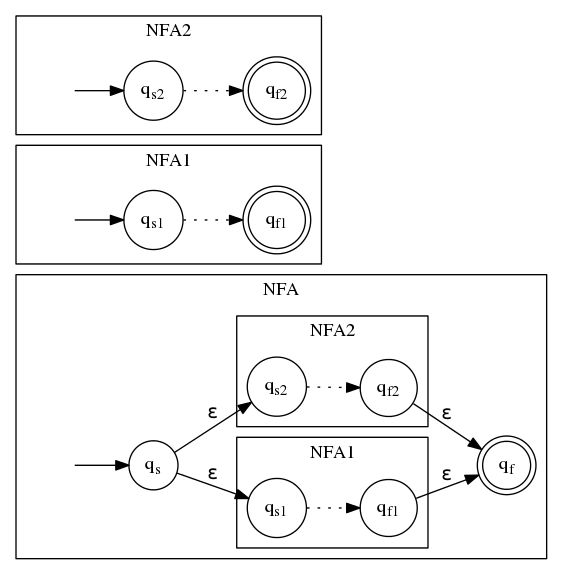
\includegraphics[width=0.5\textwidth]{assets/nfa_unie.png}      
      \caption{De unie van twee NFA's}
      \label{fig:nfa_unie}
    \end{figure}
    Formeel beschrijven we $n$ als volgt.
    \begin{itemize}
    \item $Q = Q_{1} \cup Q_{2} \cup \{ q_{s}, q_{f} \}$ waarbij $q_{s}$ en $q_{f}$ nieuwe toestanden zijn.
    \item $F = {q_{f}}$
    \item $\delta$ wordt aangepast als volgt:
      \begin{itemize}
      \item $\forall q \in Q_{i}\setminus\{q_{f_{i}}\},\ \forall x \in \Sigma_{\epsilon}:\ \delta(q,x) = \delta_{i}(q,x)$
      \item $\delta(q_{s},\epsilon) = \{q_{s1},q_{s2}\}$
      \item $\forall x \in \Sigma:\ \delta(q_{s},x) = \emptyset$
      \item $\delta(q_{f1},x) = \{q_{f}\}$ en $\delta(q_{f2},x) = \{q_{f}\}$
      \item $\forall x \in \Sigma:\ \delta(q_{f1},x) = \emptyset$, $\delta(q_{f2},x) = \emptyset$ en $\delta(q_{f},x) = \emptyset$ 
      \end{itemize}
    \end{itemize}
  \end{proof}
\end{st}

\begin{de}
  De \term{concatenatie} $n_{1}n_{2}$ van twee NFA's $n_{1}$ en $n_{2}$ is de NFA $n$ die de concatenatie van de talen $L_{n_{1}}$ en $L_{n_{2}}$ aanvaardt.
\end{de}

\begin{st}
  Constructie van de \term{concatenatie van NFA's}\\
  Het is steeds mogelijk om de concatenatie van twee NFA's te construeren.

  \begin{proof}
    Zij $n_{1} = (Q_{1},\Sigma,\delta_{1},q_{s1},\{q_{f1}\})$ en $n_{2} = (Q_{2},\Sigma,\delta_{2},q_{s2},\{q_{f2}\})$ twee willekeurige NFA's. We construeren nu de unie $n = n_{1}n_{2} = (O,\Sigma,\delta,q,\{q_{f}\})$ van deze NFA's.
    De informele constructie ziet u in figuur \ref{fig:nfa_concat}.
    \begin{figure}[H]
      \centering
      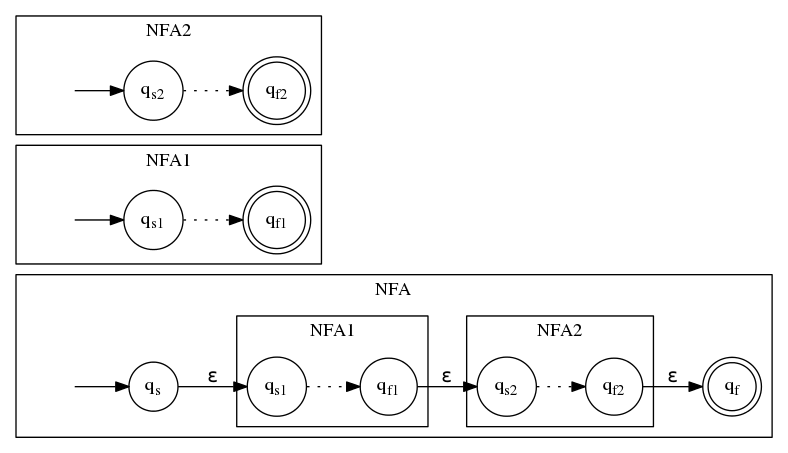
\includegraphics[width=0.7\textwidth]{assets/nfa_concat.png}      
      \caption{De concatenatie van twee NFA's}
      \label{fig:nfa_concat}
    \end{figure}
    Formeel beschrijven we $n$ als volgt.
    \begin{itemize}
    \item $Q = Q_{1} \cup Q_{2} \cup \{ q_{s}, q_{f} \}$ waarbij $q_{s}$ en $q_{f}$ nieuwe toestanden zijn.
    \item $F = {q_{f}}$
    \item $\delta$ wordt aangepast als volgt:
      \begin{itemize}
      \item $\forall q \in Q_{i}\setminus\{q_{f_{i}}\},\ \forall x \in \Sigma_{\epsilon}:\ \delta(q,x) = \delta_{i}(q,x)$
      \item $\delta(q_{s},\epsilon) = \{q_{s1}\}$
      \item $\forall x \in \Sigma:\ \delta(q_{s},x) = \emptyset$
      \item $\delta(q_{f1},\epsilon) = \{q_{s2}\}$
      \item $\delta(q_{s2},\epsilon) = \{q_{f}\}$
      \item $\forall x \in \Sigma:\ \delta(q_{f1},x) = \emptyset$, $\delta(q_{f2},x) = \emptyset$ en $\delta(q_{f},x) = \emptyset$ 
      \end{itemize}
    \end{itemize}
  \end{proof}
\end{st}

\begin{de}
  De \term{Kleene-ster} van een NFA $n'$ is de NFA $n$ die de Kleenester van de taal $L_{n'}$ aanvaardt.
\end{de}

\begin{st}
  Constructie van de \term{Kleene-ster van een NFA}\\
  Het is steeds mogelijk om de Kleene-ster van een NFA te construeren.

  \begin{proof}
    Zij $n' = (Q',\Sigma,\delta',q_{s},\{q_{f}'\})$ een willekeurige NFA. We construeren nu de Kleenester $n = (O,\Sigma,\delta,q,F)$ van deze NFA.
    De informele constructie ziet u in figuur \ref{fig:nfa_kleene}.
    \begin{figure}[H]
      \centering
      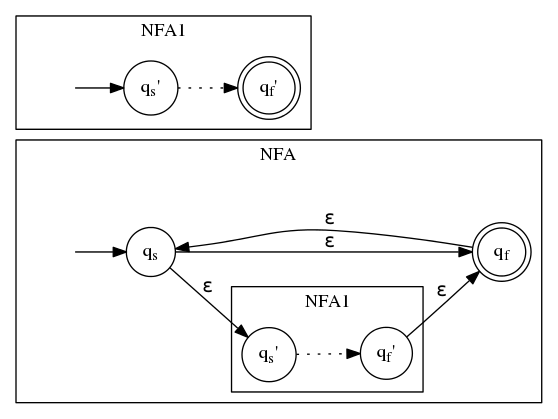
\includegraphics[width=0.5\textwidth]{assets/nfa_kleene.png}      
      \caption{De Kleenester van een NFA}
      \label{fig:nfa_kleene}
    \end{figure}
    Formeel beschrijven we $n$ als volgt.
    \begin{itemize}
    \item $Q = Q' \cup \{ q_{s}, q_{f} \}$ waarbij $q_{s}$ en $q_{f}$ nieuwe toestanden zijn.
    \item $F = {q_{f}'}$
    \item $\delta$ wordt aangepast als volgt:
      \begin{itemize}
      \item $\forall q \in Q'\setminus\{q_{f}'\},\ \forall x \in \Sigma_{\epsilon}:\ \delta(q,x) = \delta_{i}(q,x)$
      \item $\delta(q_{s},\epsilon) = \{q_{s}'\}$
      \item $\forall x \in \Sigma:\ \delta(q_{s},x) = \emptyset$
      \item $\delta(q_{f}',\epsilon) = \{q_{f}\}$
      \item $\delta(q_{f},\epsilon) = \{q_{s}\}$
      \item $\delta(q_{s},\epsilon) = \{q_{f}\}$
      \item $\forall x \in \Sigma:\ \delta(q_{f}',x) = \emptyset$ en $delta(q_{f},x) = \emptyset$
      \end{itemize}
    \end{itemize}
  \end{proof}
\end{st}

\begin{de}
  Het \term{complement} van een NFA $n$ is de NFA $n^{c}$ die het complement $L_{n}^{c}$ van de taal $L_{n}$ aanvaardt.
\end{de}

\begin{st}
  Constructie van het \term{complement van een NFA}\\
  Het is steeds mogelijk om het complement van een NFA te construeren.

  \begin{proof}
    Zij $n' = (Q',\Sigma,\delta,q_{s},F)$ een willekeurige NFA. We construeren nu het complement $n = (O,\Sigma,\delta,q_{s},F)$ van deze NFA.
    De informele constructie ziet u in figuur \ref{fig:nfa_kleene}.
    \begin{figure}[H]
      \centering
      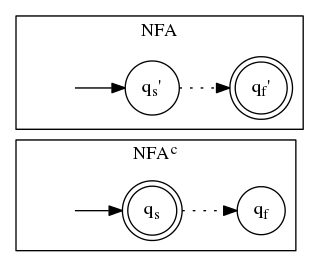
\includegraphics[width=0.5\textwidth]{assets/nfa_complement.png}      
      \caption{Het complement van een NFA}
      \label{fig:nfa_complement}
    \end{figure}
    Formeel beschrijven we $n$ als volgt.
    \begin{itemize}
    \item $Q = Q'$.
    \item $F = Q'\setminus F'$.
    \end{itemize}
  \end{proof}
\end{st}

\begin{ei}
  NFA's, uitgerust met de unie, de doorsnede, het complement en de concatenatie vormen een algebra.
  \begin{proof}
    Inderdaad, zowel de unie, de doorsnede, het complement als de concatenatie zijn inwendig.
  \end{proof}
\end{ei}

\section{Van reguliere expressie naar NFA}
\label{sec:van-reguliere-expressie-naar-nfa}

\begin{de}
  Definieer de NFA $NFA_{\epsilon}$ als $(Q, \Sigma, \delta, q_{s}, F)$.

  \begin{itemize}
  \item $Q = \{q_{s},q_{d}\}$.
  \item 
    \[ \forall q \in Q, c \in \Sigma:\ \delta(q,c) = q_{d} \]
  \item $F = \{q_{s}\}$
  \end{itemize}

  \begin{figure}[H]
    \centering
    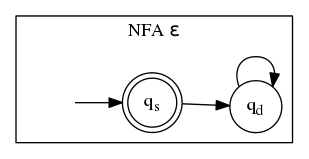
\includegraphics[width=0.3\textwidth]{assets/nfa_epsilon.png}      
    \caption{De NFA $NFA_{\epsilon}$}
    \label{fig:nfa_epsilon}
  \end{figure}
\end{de}

\begin{de}
  Definieer de NFA $NFA_{phi}$ als $(Q, \Sigma, \delta, q_{s}, \emptyset)$.

  \begin{itemize}
  \item $Q = \{q_{s}\}$
  \item 
    \[ \forall c \in \Sigma:\ \delta(q,c) = q_{s} \]
  \end{itemize}

  \begin{figure}[H]
    \centering
    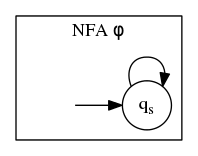
\includegraphics[width=0.2\textwidth]{assets/nfa_phi.png}      
    \caption{De NFA $NFA_{\phi}$}
    \label{fig:nfa_phi}
  \end{figure}
\end{de}

\begin{de}
  Definieer de NFA $NFA_{a}$ (met $a$ in $\Sigma$) als $(Q, \Sigma, \delta, q_{s}, F)$.

  \begin{itemize}
  \item $Q = \{q_{s},q_{f},q_{d}\}$
  \item $\delta$
    \[ \delta(q_{s}, a) = q_{f} \]
    \[ \forall c \in \Sigma\setminus\{a\}:\ \delta(q_{s}, c) = q_{d} \]
    \[ \forall c \in \Sigma:\ \delta(q_{f}, c) = q_{d}\]
    \[ \forall c \in \Sigma:\ \delta(q_{d}, c) = q_{d}\]
  \item $F = \{q_{f}\}$
  \end{itemize}

  \begin{figure}[H]
    \centering
    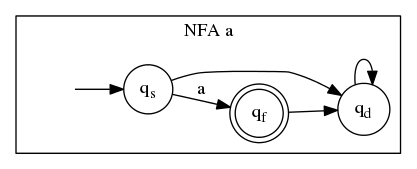
\includegraphics[width=0.4\textwidth]{assets/nfa_a.png}      
    \caption{De NFA $NFA_{a}$}
    \label{fig:nfa_a}
  \end{figure}
\end{de}

\begin{de}
  Definieer nu \term{NFA van een reguliere expressie}, samen met de vorige definitie als volgt:
  \begin{itemize}
  \item $NFA_{E_{1}E_{2}} = NFA_{E_{1}}NFA_{E_{2}}$
  \item $NFA_{(E_{1}|E_{2})} = NFA_{E_{1}} \cup NFA_{E_{2}}$
  \item $NFA_{E_{1}^{*}} = NFA_{E_{1}}^{*}$
  \end{itemize}
\end{de}

\section{NFA naar reguliere expressie}
\begin{de}
  Een gegeneraliseerde niet-deterministische eindige toestandsautomaat (\term{GNFA}) is een 5-tal $(Q,\Sigma,\delta,q_{s},q_{f}$).
  \begin{itemize}
  \item $Q$ is een eindige verzameling toestanden.
  \item $\Sigma$ is een alfabet.
  \item $\delta$ is de overgangsfunctie.
  Merk op dat deze functie twee staten als argument neemt in plaats van een staat en een symbool.
    \[
    \delta: Q\setminus\{q_{s}\} \times Q\setminus\{q_{f}\} \rightarrow RegEx_{\Sigma}
    \]
  \item $q_{s}$ is de starttoestand.
  \item $q_{f}$ is de aanvaardbare eindtoestand.
  \end{itemize}
  Een GNFA heeft de volgende (informele) eigenschappen.
  \begin{itemize}
  \item Er is precies een eindtoestand en die is verschillend van de eindtoestand.
  \item Er is precies een boog van elke toestand naar de eindetoestand
  \item Uit de eindtoestand vertrekken geen pijlen.
  \item Tussen elke twee toestanden (behalve de begin- en eindtoestand) vertrekt precies \'e\'en boog in beide richtingen
  \item Er is precies \'e\'en boog van elke toestand (behalve de begin- en eindtoestand) naar zichzelf.
  \item De bogen hebben een reguliere expressie als label.
  \end{itemize}
\end{de}

\begin{de}
  Een string $s$ wordt aanvaard door een GNFA als er een rij reguliere expressies $E_{1},E_{2},\dotsc,E_{n}$ bestaat zodat $s$ wordt aanvaard door de concatenatie van die rij reguliere expressies en zodat die reguliere expressies een pad $t_{1},t_{2},\dotsc,t_{n+1}$ vormen in de GNFA. 
  \begin{itemize}
  \item $t_{1} = q_{s}$
  \item $\delta(t_{i},t_{i+1}) = E_{i}$
  \item $t_{n+1} = q_{f}$
  \end{itemize}
\end{de}

\begin{st}
  \label{st:nfa-naar-regex}
  We kunnen iedere NFA omzetten in een reguliere expressie die dezelfde taal bepaalt.
  
  \begin{proof}
    \begin{enumerate}
    \item Maak van de NFA een GNFA:\\
      Voer een nieuwe begintoestand, en een nieuwe unieke eindtoestand.
      Teken een $\epsilon$-boog van de nieuwe begintoestand naar de oude, alsook een $\epsilon$-boog van de oude eindtoestand naar de nieuwe.
      Teken alle ontbrekende bogen met een $\phi$ (deze mogen toch niet gevolgd worden).
      Het is evident dat deze GNFA dezelfde taal bepaalt als de originele NFA.
    \item Reduceer de GNFA:\\
      Kies een willekeurige toestand $X$ verschillend van de begin- of eindtoestand.
      Verwijder $X$ als volgt: Kies toestanden $A$ en $B$ zodat er bogen zijn van $A$ naar $B$ met reguliere expressie $E_{4}$, van $A$ naar $X$ met $E_{1}$, van $X$ naar zichzelf met $E_{2}$ en van $X$ naar $B$ met $E_{3}$.
      \begin{figure}[H]
        \centering
        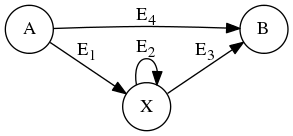
\includegraphics[width=0.3\textwidth]{assets/nfa-gnfa1.png}
        \text{\hspace{1cm}wordt\hspace{1cm}}
        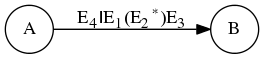
\includegraphics[width=0.3\textwidth]{assets/nfa-gnfa2.png}   
        \label{fig:nfa-gnfa}
      \end{figure}
      Vervang het label op de boog van $A$ naar $B$ door $(E_{4}|E_{1}E_{2}^{*}E_{3})$.
      Doe dit voor alle koppels $A$ en $B$ ten opzichte van $X$ en verwijder tenslotte $X$.
      \[
      \forall a,b,c: ((\delta(a,b)=E_{4})\wedge (\delta(a,x)=E_{1})\wedge (\delta(x,x)=E_{2})\wedge (\delta(x,b)=E_{3})) 
      \]
      \[
      \Rightarrow \delta'(a,b)=(E_{4}|E_{1}E_{2}^{*}E_{3})
      \]
      Itereer dit proces tot enkel nog de begin- en eindtoestand overblijven.
      Dit proces verandert de bepaalde taal niet.
      Noem de machine voor het proces $GNFA_{voor}$ en na het proces $GNFA_{na}$.
      Kies nu een willekeurige string $s \in \Sigma^{*}$.
      \begin{itemize}
      \item
        Als $s$ aanvaard werd door $GNFA_{voor}$ met een pad dat $X$ niet bevat, dan wordt $s$ door datzelfde pad in $GNFA_{na}$ aanvaard.
        Als het pad $X$ wel bevat, dan zijn er toestanden $A$ en $B$ zodat $AX^{n}B$ met $n\in \mathbb{N}_{0}$ een opeenvolging is in het pad. De reguliere expressie op de bogen $AX$, $XX$, $XB$ zijn $E_{1}$, $E_{2}$ en $E_{3}$. Bijgevolg kost van $A$ naar $B$ gaan langs $X$ een stukje string dat voldoet aan $E_{1}E_{2}^{*}E_{3}$. Die reguliere expressie staat in $GNFA_{na}$ in de boog $AB$, dus $s$ wordt ook aanvaard door $GNFA_{na}$.
      \item
        Als $s$ aanvaard wordt door $GNFA_{na}$ dan bevat het acceptatiepad alleen maar toestanden verschillend van $X$. Op een boog van $A$ naar $B$ staat de reguliere expressie $E_{4}|E_{1}E_{2}^{*}E_{3}$. Die reguliere expressie gebruiken kost een stukje string dat voldoet aan $E_{4}$ of $E_{1}E_{2}^{*}E_{3}$. In $GNFA_{voor}$ komt dat overeen met ofwel boog $AB$ volgen, ofwel $AX$, gevolgd door $n$ keer $XX$ en $XB$. Dit houdt in dat de string ofwel het pad langs $X$ nodig had, ofwel het pad zonder $X$, langs $A$ en $B$. In beide gevallen aanvaardt $GNFA_{voor}$ ook $s$.
      \end{itemize}
    \item Bepaal de reguliere expressie.\\
      De overblijvende GNFA heeft nu precies twee toestanden met \'e\'e boog daartussen.
      De reguliere expressie $E$ van die boog is precies de reguliere expressie die we zochten.
    \end{enumerate}
  \end{proof}
\end{st}

\begin{gev}
  \label{gev:reguliere-taal-NFA}
  Elke reguliere taal wordt bepaald door een NFA.
  
  \begin{proof}
    Elke reguliere taal wordt bepaald door een reguliere expressie.\footnote{Zie eigenschap \ref{ei:reguliere-taal-expressie}.}
    Elke reguliere expressie kan bovendien omgezet worden in een NFA die dezelfde taal bepaalt.\footnote{Zie stelling \ref{st:nfa-naar-regex}.}
  \end{proof}
\end{gev}

\begin{ei}
  Er bestaat een isomorfisme tussen de algebra van NFA's en de algebra van Reguliere expressies.

  \begin{proof}
    Beschouw de vier bewerkingen in de algebra van reguliere expressies: unie $\cup_{R}$, concatenatie $\cdot_{R}$, complement $^{c}_{R}$ en doorsnede $\cap_{R}$.
    Er bestaan overeenkomstige bewerkingen in de algebra van NFA's: unie $\cup_{N}$, concatenatie $\cdot_{N}$, complement $^{c}_{R}$ en doorsnede $\cap_{N}$.
    Bovendien bestaat er een functie die een willekeurige reguliere expressie afbeeldt op een reguliere expressie die dezelfde taal bepaalt.\footnote{Zie stelling \ref{st:nfa-naar-regex}.}
    Er bestaat dus een eenvoudig isomorfisme tussen deze twee algebra's.
  \end{proof}
\end{ei}

\section{Deterministische eindige toestandsautomaten}
\begin{de}
  Een deterministische eindige toestandsautomaat (\term{DFA}) is een 5-tal $(Q,\Sigma,\delta,q_{s}F)$
  \begin{itemize}
  \item $Q$ is een eindige verzameling toestanden.
  \item $\Sigma$ is een alfabet.
  \item $\delta$ is de parti\"ele overgangsfunctie van de automaat.
  \[ \delta: Q \times \Sigma \rightarrow Q \]
  \item $q_{s} \in Q$ is de starttoestand.
  \item $F \subseteq Q$ is de verzameling aanvaardbare eindtoestanden.
  \end{itemize}
\end{de}

\begin{de}
  We kunnen $\delta(q,a)$ afkorten als $q_{a}$ wanneer de $\delta$ die bedoeld wordt duidelijk is.  
\end{de}

\begin{de}
  Een string $s$ wordt aanvaard door een DFA als de opeenvolgende symbolen $s_{1}s_{2}\dotsc s_{n}$ van $s$ een pad $t_{1},t_{2},\dotsc,t_{n}$ vormen in de DFA.
  \begin{itemize}
  \item $t_{1} = q_{s}$
  \item $\delta(t_{i},s_{i}) = t_{i+1}$
  \item $t_{n+1} \in F$
  \end{itemize}
\end{de}

\begin{de}
  De \term{taal} $L_{M}$ \term{bepaald door een DFA} $D$ bevat alle strings die $D$ aanvaardt, en geen andere strings.
\end{de}

\begin{de}
  Twee DFA's $d_{1}$ en $d_{2}$ zijn equivalent als ze dezelfde taal bepalen.
  \[ d_{1} \sim d_{2} \]
\end{de}

\begin{st}
  Elke NFA kan omgezet worden in een DFA die dezelfde taal bepaalt.
  
  \begin{proof}
    Zij $N$ een willekeurige NFA.
    \[ N = (Q_{n},\Sigma,\delta_{n},q_{n},F_{n}) \]
    We construeren nu een DFA $D$ die dezelfde taal bepaalt.
    \[ D = (Q_{d},\Sigma,\delta_{d},q_{d},F_{d}\]
    De toestanden $Q_{d}$ voor de DFA zullen elk overeen komen met een verzameling toestanden uit de NFA.
    \[ Q_d = \mathcal{P}(Q_{n})\]
    Een eindtoestand in de DFA komt steeds overeen met een verzameling die een eindtoestand van de NFA bevat.
    \[ \forall q\in Q_{d}:\ q\in F_{d}\ \Rightarrow \exists q' \in F_{n}: q' \in q\]
    Nu rest er ons nog $\delta_{d}$ te construeren.
    \[
    \delta_{d}:\ (\mathcal{P}(Q_{n}) \times \Sigma) \rightarrow \mathcal{P}(Q_{n})
    \]
    We voeren een een afbeelding $eb$ in die elke staat in $Q_{n}$ afbeeldt op al haar epsilon bereikbare toestanden in $Q_{n}$.
    \[ eb: Q_{n} \rightarrow \mathcal{P}(Q_{n}) \]
    \begin{itemize}
    \item $eb(q)$ is de verzameling toestanden die met een aantal $\epsilon$-bogen bereikbaar is vanuit $q$.
    \item $eb(Q)$ defineren we als volgt:
      \[ ex(Q) = \bigcup_{q\in Q} eb(q)\]
    \item $\delta_{n}(Q)$ definieren we als volgt:
      \[ \delta_{n}(Q) = \bigcup_{q\in Q} \delta(q,a) \]
    \end{itemize}
    We construeren nu $\delta_{d}$:
    \[ \forall Q\in Q_{d}:\ \delta_{d}(Q,a) = eb(\delta_{n}(Q,a)) \]
    In woorden teken een boog in de DFA van elke verzameling toestanden naar de verzameling toestanden die epsilon-bereikbaar zijn vanuit die verzameling.
    Tenslotte definieren we nog de begintoestand van $D$.
    \[ q_{sd} = eb(q_{sn}) \]
  \end{proof}
\end{st}

\begin{st}
  \label{gev:reguliere-taal-DFA}
  Elke reguliere taal wordt bepaald door een DFA
  
  \begin{proof}
    Elke reguliere taal wordt bepaald door een NFA\footnote{Zie gevolg \ref{gev:reguliere-taal-NFA}.}
    Bovendien kan elk NFA omgezet worden in een DFA die dezelfde taal bepaalt.
  \end{proof}
\end{st}

\begin{de}
  Voor elke DFA $(Q,\Sigma,\delta,q_{s},F)$ kunnen we $\delta:\ Q \times \Sigma$ uitbreiden naar $\delta^{*}:\ Q\times \Sigma^{*}$.
  \begin{itemize}
  \item $\delta^{*}(q,\epsilon) = q$
  \item $\exists \delta(q,a) \Rightarrow \delta^{*}(q,aw) = \delta^{*}(\delta(q,a),w)$
  \end{itemize}
\end{de}

\begin{st}
  \label{st:delta-ster-identiteit}
  Voor elke DFA $(Q,\Sigma,\delta,q_{s},F)$ met een uitgebreide $\delta$: $\delta^{*}$ geldt de volgende gelijkheid:
  \[
  \delta^{*}(q,wa) = \delta(\delta^{*}(q,w),a)
  \] 
  
  \begin{proof}
    We bewijzen dit door inductie op de lengte $n$ van $w$.
    \begin{itemize}
    \item De bewering geldt voor $n=0$ ($w$ is dan de lege string.):
      \[ \delta^{*}(q,wa) = \delta^{*}(q,\epsilon a) = \delta^{*}(q,a\epsilon) = \delta^{*}(\delta(q,a),\epsilon) = \delta(q,a) = \delta(\delta^{*}(q,\epsilon),a) \]
    \item Stel dat de bewering geldt voor een bepaalde $n=k$.
    \item Als de bewering geldt voor een bepaalde $n=k$, dan geldt ze ook voor $n=k+1$.
      Kies een $w$ van lengte $k+1$ en noem het eerste symbool van $w$ $b$.
      De rest van $w$ noemen we dan $w'$.
      \[ w = w'b \]
      Nu kunnen we de bewering rechtstreeks bewijzen voor een willekeurig symbool $a$.
      \[
      \begin{array}{rll}
        \delta^{*}(q,wa) &= \delta^{*}(q,bw'a) &\\
                         &= \delta^{*}(\delta(q,b),w'a) &\\
                         &= \delta(\delta^{*}(\delta(q,b),w'),a) &=\delta(\delta^{*}(q,w),a) 
      \end{array}
      \]
    \end{itemize} 
    Als gevolg van het principe van inductie geldt de bewering voor elke $n\in \mathbb{N}$.
  \end{proof}

\end{st}

\begin{st}
  \label{st:dfa-totale-overgangsfunctie}
  Als een DFA $(Q,\Sigma,\delta,q_{s},F)$ een overgangsfunctie heeft die niet totaal is, met andere woorden, niet voor elk symbool is er in elke staat een boog, dan hoeven we hoogstens \'e\'en staat toe te voegen om een equivalente DFA te maken met een totale overgangsfunctie.

  \begin{proof}
   Kies een willekeurige DFA $D = (Q,\Sigma,\delta,q_{s},F)$ met een niet-totale overgangsfunctie.
   Maak nu een nieuwe, onaanvaardbare staat $q_{t}$, en vervolledig de overgangsfunctie $\delta$ door een koppel $((q,a),q_{t})$ toe te voegen voor elk koppel $(q,a)$ waarvoor $\delta$ onbepaald is om $\delta'$ te bekomen.
   Voeg bovendien aan $\delta'$ ook nog voor elke symbool $s$ uit het alfabet $\Sigma$ het volgende koppel toe:
   \[ ((q_{t},s),q_{t}) \]
   Nu is de overgangsfunctie $\delta'$ totaal.
   De nieuwe DFA $D' = (Q\cup\{ q_{t} \},\Sigma,\delta',q_{s},F)$ is nu bovendien equivalent met $D$ door hoogstens \'e\'en staat toe te voegen.
  \end{proof}
\end{st}

\section{Minimale DFA}
\begin{de}
  Twee toestanden $p$ en $q$ van een DFA $(Q,\Sigma,\delta,q_{s},F)$ zijn \term{$f$-gelijk} $p\sim q$ als het volgende geldt:
  \[
  \forall w \in \Sigma^{*}:\ \delta^{*}(p,w) \in F \Leftrightarrow \delta^{*}(q,w) \in F
  \]
  In woorden: dezelfde strings worden aanvaard vanuit beide toestanden $p$ en $q$.
\end{de}

\begin{de}
  Twee toestanden $p$ en $q$ van een DFA $(Q,\Sigma,\delta,q_{s},F)$ zijn \term{$f$-verschillend} als ze niet $f$-gelijk zijn. 
\end{de}

\begin{opm}
  $f$-gelijkheid kunnen we ook definieren voor NFA's, maar dan wordt $f$-verschillend moeilijk te definieren.
\end{opm}

\begin{ei}
  $f$-gelijkheid is een equivalentierelatie, en bepaalt dus een partitionering van een verzameling staten $Q$ van een $DFA$.

  \begin{proof}
    Inderdaad, de relatie ``A is $f$-gelijk met B'' is reflexief, transitief en symmetrisch.
  \end{proof}
\end{ei}

\begin{al}
  \label{al:dfa-minimalisatie}
  \emph{$f$-gelijke toestanden vinden.}\\
  Gegeven een DFA $(Q,\Sigma,\delta,q_{s},F)$, zoeken we de partitionering van $D$ in verzamelingen van $f$-gelijke toestanden.

  \begin{figure}[H]
    \centering
    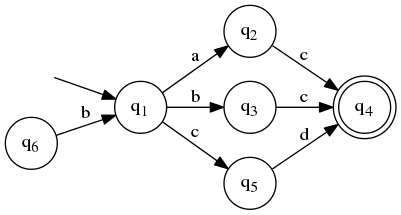
\includegraphics[width=0.4\textwidth]{assets/dfa_minimalisatie-1.png}     
    \caption{Een niet-minimale DFA}
    \label{fig:dfa-minimalisatie-1}
  \end{figure}

  \subsubsection{Pre-init}
  \textit{
    Elke staat die niet bereikbaar is vanaf $q_s$ kunnen we zonder meer verwijderen
  }

  Ga voor elke staat $q\in Q$ na of $q$ bereikbaar is vanaf $q_{s}$, zo nee, verwijder $q$.

  \begin{figure}[H]
    \centering
    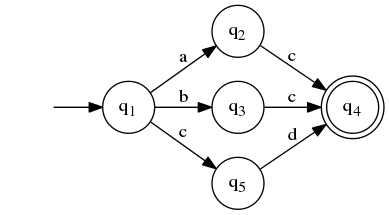
\includegraphics[width=0.4\textwidth]{assets/dfa_minimalisatie-2.png}     
    \caption{Een niet-minimale DFA zonder nutteloze staten}
    \label{fig:dfa-minimalisatie-2}
  \end{figure}

  \subsubsection{Init}
  \textit{
    Kies een toestand $p$ die geen eindtoestand is.
    $p$ is zeker $f$-verschillend van elke eindtoestand.
    Alle andere paren zijn nog onbeslist.
  }

  Beschouw de ongerichte graaf $G(Q,E)$ met de toestanden $Q$ als knopen en noem $E$ de bogen van $G$.
  De graaf heeft bovendien een label voor elke boog.
  Begin met een lege verzameling $E$.
  Voeg nu voor elk paar knopen $p$ en $q$ waarvan er precies \'e\'en een aanvaardbare toestand is een boog toe tussen $p$ en $q$.
  \[ \forall p,q:\ p \in F \oplus q \in F:\ (p,q,\epsilon) \in E \]

  \begin{figure}[H]
    \centering
    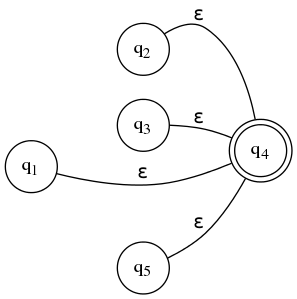
\includegraphics[width=0.4\textwidth]{assets/dfa_minimalisatie-3.png}     
    \caption{De graaf $V$ na de initialisatie van het minimalisatie algoritme.}
    \label{fig:dfa-minimalisatie-3}
  \end{figure}

  \subsubsection{Repeat}
  \textit{
    Kies een paar toestanden $p$ en $q$ dat nog onbeslist is.
    Stel dat er een symbool $a$ bestaat zodat je met dat symbool van $p$ en van $q$ gaat naar twee $f$-verschillende toestanden, dan beslis je dat $p$ en $q$ $f$-verschillend zijn.
  }

  Als er twee knopen $p$ en $q$ zijn waarvoor het volgende geldt:
  \begin{itemize}
  \item Er is geen boog tussen $p$ en $q$.
    \[ \not\exists (p,q,\_) \in E \]
  \item Er bestaat een symbool zodat je met dat symbool vanuit $p$ en vanuit $q$ een toestand kan bereiken waartussen een boog is.
    \[ \exists a \in \Sigma:\ \exists(p_{a},q_{a},\_) \in V \]
  \end{itemize}
  Kies een symbool $a$ waarvoor $(p_{a},q_{a},\_)$ al een boog is van $G$ en voeg de boog $(p,q,a)$ toe.
  \[ (p,q,a) \in E \]
  Het is hier noodzakelijk om op te merken dat we de overgangsfunctie $\delta$ eigenlijk eerst totaal moeten maken.\footnote{Zie stelling \ref{st:dfa-totale-overgangsfunctie}.}

\question{foutje in boek?: figuur 2.13 tweede prentje. Moet je de (impliciete) trash state meerekenen?}
  \begin{figure}[H]
    \centering
    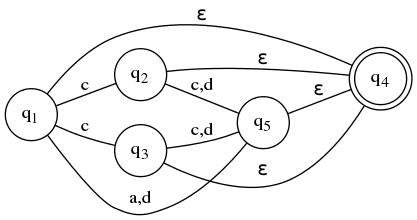
\includegraphics[width=0.4\textwidth]{assets/dfa_minimalisatie-4.png}     
    \caption{De graaf $V$ na alle repeat stappn van het minimalisatie algoritme.}
    \label{fig:dfa-minimalisatie-4}
  \end{figure}

  \subsubsection{Consolidate}
  \textit{
    Voor elk paar toestanden $p$ en $q$ waarvoor je nog niet beslist had, beslis je nu dat $p$ en $q$ $f$-gelijk zijn.
    Gebruik deze equivalentierelatie om $Q$ te partitioneren.
  }  

  Bouw nu de complementsgraaf $G^{c}$ van $G$.
  In $G^{c}$ is er een boog tussen elke twee knopen waartussen in $G$ geen boog was.
  Elke component van $G^{c}$ stelt nu een verzameling in de partitie van $Q$ voor in $f$-gelijke disjucnte deelverzamelingen.

  \begin{figure}[H]
    \centering
    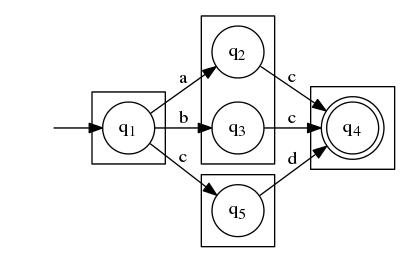
\includegraphics[width=0.4\textwidth]{assets/dfa_minimalisatie-5.png}     
    \caption{De partitionering van Q op het einde van het minimalisatie algoritme.}
    \label{fig:dfa-minimalisatie-5}
  \end{figure}

\end{al}
\begin{st}
  Bovenstaand algoritme (\ref{al:dfa-minimalisatie}) is eindig en correct.
  \begin{proof}
    \begin{itemize}
    \item Eindigheid.\\
    Het aantal knopen in $G$ is eindig omdat de DFA een eindig aantal toestanden heeft, en het aantal is dat $\frac{N(N-1)}{2}$ met $N$ het aantal knopen van $G(Q,E)$.
    Elk van die bogen wordt bovendien een eindig aantal keer overlopen.
    \item Correctheid.\\
      We bewijzen volgende bewering voor de graaf $G$ na de ``repeat'' stap:
      \[ (p,q,\_) \in E \Leftrightarrow p \text{ en } q \text { zijn } f\text{verschillend.}\]
      \begin{itemize}
      \item $\Rightarrow$\\
        Als $(p,q,l)$ een boog is van $G$, dan zijn er twee mogenlijkheden.
        Ofwel is het een $\epsilon$-boog: $l=\epsilon$, ofwel is het een boog met een symbool als label: $l = a \in \Sigma$.
        Als het een $\epsilon$-boog is, dan zijn $p$ en $q$ $f$-verschillend omdat de lege string de DFA bijvoorbeeld niet in een zelfde soort toestand zou brengen.
        \[ \delta^{*}(p,\epsilon) \in F \not\Leftrightarrow \delta^{*}(q,\epsilon) \]
        Als het geen $\epsilon$-boog is, volg dan bestaat er een string $w$ die de DFA niet in een zelfde soort toestand brengen.
        \[ \exists w\in \Sigma^{*}:\ \delta^{*}(p,w) \in F \not\Leftrightarrow \delta^{*}(q,w) \]
        Dit omdat die string $w$ de DFA in respectievelijke toestanden zou brengen waartussen in $G$ een $\epsilon$-boog is.
        \[ \exists w\in \Sigma^{*}:\  \delta^{*}(p_{w},\epsilon) \in F \not\Leftrightarrow \delta^{*}(q_{w},\epsilon) \]
      \item $\Leftarrow$\\
        Als $p$ en $q$ $f$-verschillend zijn, dan bestaat er een string $w\in \Sigma^{*}$ die de DFA vanuit $p$ in een aanvaarbare toestand brengt, maar $q$ niet of omgekeerd.
        \[ \exists w \in \Sigma^{*}: \delta^{*}(p,w) \in F \not\Leftrightarrow \delta^{*}(q,w) \]
        Als die string $w$ leeg is, dan bestaat er sinds de initialisatiestap al een boog tussen $q$ en $w$. Als die string niet leeg is, dan kan $w$ geschreven worden als $w = vz$ met $v$ het eerste deel van $w$ en $z$ een symbool.
        \[ \exists v\in \Sigma^{*}, z \in \Sigma: w = vz \]
        Nu geldt het volgende:\footnote{Zie stelling \ref{st:delta-ster-identiteit}.}
        \[ \delta^{*}(p,w) = \delta(\delta^{*}(p,v),z) \text{ en } \delta^{*}(q,w) = \delta(\delta^{*}(q,v),z)\]
        Er is dus een boog tussen $\delta^{*}(p,v)$ en $\delta^{*}(q,v)$ dankzij de ``repeat'' stap.
        Dit betekent dat we het laatste symbool weer kunnen schrappen tot we uitkomen op een boog tussen $\delta^{*}(p,\epsilon)$ en $\delta^{*}(q,\epsilon)$.
\question{Iets meer uitleg hier..?}
      \end{itemize}
    \end{itemize}
  \end{proof}
\end{st}

\begin{de}
  Een DFA $D = (Q,\Sigma,\delta,q_{s},F)$ is \emph{minimaal} als er geen DFA $D'$ bestaat met strikt minder toestanden.
\end{de}

\begin{st}
  Als een DFA $(Q,\Sigma,\delta,q_{s},F)$ geen onbereikbare toestanden heeft, en elke twee toestanden $f$-verschillend zijn, dan bestaat er geen machine met strikt minder toestanden die dezelfde taal bepaalt.

  \begin{proof}
    Bewijs uit het ongerijmde.\\
    Zij $D = (Q,\Sigma,\delta,q_{s},F)$ een DFA zonder onbereikbare toestanden, waarbij elke twee toestanden $f$-verschillend zijn.
    Stel nu dat er een DFA $D' = (Q',\Sigma,\delta',q_{s},F')$ bestaat die strikt minder toestanden heeft dan $D$. We bewijzen nu dat er dan minstens \'e\'en string is waarwoor $D$ niet in dezelfde soort toestand eindigt als $D'$.
    
    Elke toestand van $D$ is bereikbaar.
    Er bestaat dus een string voor elke toestand die een pad naar die toestand zou volgen.
    \[ \forall q\in Q, \exists s\in \Sigma^{*}:\ \delta^{*}(q_{s},s) = q \]
\question{ op pagine 34 in het boek staat $p_{s}$, wat is dit? }
    Omdat $D'$ minder toestanden heeft dan $D$ moet er minstens twee van de strings die in $D$ in verschillende toestanden zouden eindigen in dezelfde toestand eindigen.
    \[ \exists s_{1},s_{2} \in \Sigma: (\delta^{*}(q_{s},s_{1}) \neq \delta^{*}(q_{s},s_{2})) \wedge (\delta'^{*}(q_{s},s_{1}) = \delta'^{*}(q_{s},s_{2})) \]
    Vermits die toestanden van $D$ $f$-verschillend zijn bestaat er een string $v\in \Sigma^{*}$ die de machine vanuit die toestanden niet in dezelfde soort toestand brengt:
    Noem die staten $\delta^{*}(q_{s},s_{1}) = q_{1}$ en $\delta^{*}(q_{s},s_{2}) = q_{2}$.
    \[ (\delta^{*}(q_{1},v) \in F) \oplus (\delta^{*}(q_{2},v) \in F) \]
    Dit houdt precies het volgende in:
    \[ (\delta^{*}(q_{s},s_{1}v) \in F) \oplus (\delta^{*}(q_{s},s_{2}v) \in F) \]
    $D$ accepteert dus precies \'e\'en van de twee strings $s_{1}v$ en $s_{2}v$.
    We bekijken nu wat $D'$ met deze strings zou doen.
    \[ \delta'^{*}(q_{s},s_{1}v) = \delta'^{*}(\delta'^{*}(q_{s},s_{1}),v) = \delta'^{*}(\delta'^{*}(q_{s},s_{2}),v) = \delta'^{*}(q_{s},s_{2}v) \]
    $D'$ zou ofwel zowel $s_{1}v$ als $s_{2}v$ accepteren, ofwel geen van beide.
    In beide gevallen is dit niet hetzelfde gedrag als $D$.
    $D$ en $D'$ kunnen dus niet dezelfde taal bepalen.
  \end{proof}
\end{st}

\begin{gev}
  We kunnen de minimale DFA $D = (Q,\Sigma,\delta,q_{s},F)$ van $D' = (Q',\Sigma,\delta',q_{s}',F')$ dus construeren nadat we $Q'$ hebben gepartitioneerd in disjuncte deelverzamelingen van $f$-gelijke toestanden.

  \begin{proof}
    Bekijk de partitie $P = \{Q_{1},\dotsc,Q_{n}$ van $Q'$ als de nieuwe verzameling staten.
    \[ Q = P \]
    De nieuwe overgangsfunctie ziet er nu als volgt uit:
    \[ \forall a \in \Sigma:\ \delta(Q_{i},a) = Q_{j} \text{ zodat } \exists q \in Q_{j}:\ \delta(q,a) \in Q_{j} \]
    Het maakt niet uit welke $q\in Q_{j}$ er gekozen werd omdat voor elke keuze van $q$ $\delta(q,a)$ in dezelfde deelverzameling van $P$ zit (anders zouden de toestanden in $Q_{j}$ $f$-verschillend zijn).
    De nieuwe starttoestand is de verzameling waar $q_{s}$ in zit.
    \[ q_{s} \in q_{s}'\]
    $F$ is nu de unie van de verzamelingen van aanvaardbare staten $F$ van $D'$.
    $D$ bepaalt nu dezelfde taal als $D'$.
    Dat de staten in elke $Q_{i}$ $f$-gelijk zijn maakt immers net dat het niet uitmaakt in welke van de staten $Q_{i}$ de automaat een string afgaat.
    Alle toestanden van $D$ zijn nu dus onderling $f$-verschillend.
    Als de toestanden $Q_{i}$ immers $f$-gelijk waren, dan waren het geen verschillende verzamelingen geworden in het algoritme om $Q$ te partitioneren.
    Bijgevolg is $D$ minimaal.
  \end{proof}
\end{gev}

\begin{de}
  Twee DFA's $(Q_{1},\Sigma,\delta_{1},q_{s1},F_{1})$ en $(Q_{2},\Sigma,\delta_{2},q_{s2},F_{2})$ zijn isomorf als er een bijectie $b:\ Q_{1} \rightarrow Q_{2}$ bestaat zodat de volgende beweringen gelden:
  \begin{itemize}
  \item $b(F_{1}) = F_{2}$
  \item $b(q_{s1}) = q_{s2}$
  \item $b(\delta_{1}(q,a)) = \delta_{2}(b(q),q)$
  \end{itemize}
  Twee isomorfe DFA's bepalen bovendien dezelfde taal.
\end{de}


\section{Myhill-Nerode relaties op $\Sigma$}
\label{sec:myhill-nerode-relaties}

\subsection{Partities van $\Sigma^{*}$}
\label{sec:partities-van-sigma-ster}

\begin{de}
  Definieer de functie $reach(q)$ van een DFA $(Q,\Sigma,\delta,q_{s},F)$ als alle strings waarvoor de automaat in staat $q$ belandt.
  \[
  reach(q) = \{ w \in \Sigma^{*}\ |\ \delta^{*}(q_{s},w) = q \}
  \]
\end{de}

\begin{st}
  De taal $reach(q)$ van een DFA $D = (Q,\Sigma,\delta,q_{s},F)$ is regulier voor elke $q$.
  
  \begin{proof}
    Inderdaad, construeer een nieuwe automaat $D'$ vanuit $D$ waarin enkel $q$ een accepterende eindtoestand is.
    $reach(q)$ is nu de taal bepaald door $D'$. $D'$ aanvaardt immers enkel de strings waarvoor $D$ (en dus $D'$, want we hebbn $\delta$ niet veranderd) in $q$ zou belanden.
  \end{proof}
\end{st}

\begin{st}
  De verzameling $R$ is een partitie van $\Sigma^{*}$ is een partitie van $\Sigma^{*}$ als elke toestand bereikbaar is.
  \[ R = \{ reach(q)\ |\ q \in Q \} \]

  \begin{proof}
    Kies een willekeurige DFA $D = (Q,\Sigma,\delta,q_{s},F)$ en een staat $q\in Q$.
    We gaan elke eigenschap van een partitie na.\footnote{Zie definitie \ref{de:partitie}.}
    \begin{itemize}
    \item $reach(q)$ is niet leeg.\\
      We moeten er hier van uitgaan dat de overgangsfunctie $\delta$ van $D$ totaal is.
      Dit kunnen we zonder verlies van algemeenheid.\footnote{Zie stelling \ref{st:dfa-totale-overgangsfunctie}.}
      Elke string $s\in \Sigma$ die we als invoer kunnen geven aan $D$ belandt zeker in een staat $q'$ zonder dat de automaat vast loopt.
      Nu geldt dat elke staat bereikt zal worden door minstens \'e\'en string als elke toestand bereikbaar is.
      $D$ kan immers ook gezien worden als een NFA zonder $\epsilon$ bogen (etc...). Wanneer we die NFA omzetten naar een reguliere expressie via een GNFA krijgen we een reguliere expressie zonder $\phi$'s. Er bestaat dus altijd minstens \'e\'en string die in $q$ belandt voor elke $q$.
    \item De verzamelingen in $R$ zijn onderling disjunct.
      Deze uitspraak is equivalent met de volgende: ``De DFA kan slechts in \'e\'en toestand belanden voor elke string $s\in\Sigma^{*}$''. Dit klopt omdat we het over \emph{deterministische} automaten hebben.
    \item De unie van alle verzamelingen in $R$ vormt $\Sigma^{*}$.
      Deze uitspraak is equivalent met de volgende: ``Er zijn geen strings $s\in \Sigma^{*}$ waarvoor de DFA $D$ niet in een staat van $Q$ belandt.''
      Inderdaad, het resultaat de overgangsfunctie $\delta$ blijft steeds binnen $Q$ als ze totaal is.
    \end{itemize}
  \end{proof}
\end{st}

\begin{gev}
  De partitie $R$ bepaalt de Equivalentierelatie ``voor zowel A als B belandt de automaat $D$ in dezelfde staat $q$'': $\sim_{D}$.
  \[ x \sim_{D} y \Leftrightarrow \delta^{*}(q_{s},x) = \delta^{*}(q_{s},y) \]

  \begin{proof}
    Inderdaad, $R$ is een partitie en elke partitie bepaalt een equivalentierelatie.\footnote{Zie stelling \ref{st:verband-partitie-equivalentierelatie}.}
  \end{proof}
\end{gev}

\begin{de}
  \label{de:mn-relatie}
  Een \term{Myhill-Nerode relatie} voor een taal $L$ over een alfabet $\Sigma$ is een relatie $\sim_{DFA}$ op $L$ met de volgende eigenschappen:
  \[ \sim_{DFA} \subseteq L \times L:\ l_{1} \sim_{DFA} l_{2}\]
  \[ \sim_{DFA} \text{ is } MN(L) \]
  \begin{itemize}
  \item $\sim_{DFA}$ is rechts congruent:
    \[ \forall x,y \in \Sigma^{*}, a \in \Sigma:\ x \sim_{DFA} y \Rightarrow (xa) \sim_{DFA} (ya) \]
  \item $\sim_{DFA}$ verfijnt $\sim_{L}$:
    \[ \forall x,y \in \Sigma^{*}, \forall L\in \mathcal{P}(\Sigma^{*}):\ x \sim_{DFA} y \Rightarrow x \sim_{L} y\]
    In woorden: ``Als $x \sim_{DFA} y$ zitten ofwel zowel $x$ als $y$ in $L$, ofwel geen van beide.''
  \item Het aantal equivalentieklassen van $\sim_{DFA}$ is eindig.
    We zeggen: ``De index van $\sim_{DFA}$ is eindig.''.
  \end{itemize}
\end{de}

\begin{st}
  \label{st:mn-relatie-is-equivalentierelatie}
  Elke Myhill-Nerode relatie $\sim$ voor een taal $L$ is over een alfabet $\Sigma$ is een equivalentierelatie.
  \begin{proof}
    Inderdaad, $\sim$ is reflexief, transitief en symmetrisch.
  \end{proof}
\end{st}

\begin{st}
  Voor elke DFA $D = (Q,\Sigma,\delta,q_{s},F)$ is de relatie $\sim_{D}$ een Myhill-Nerode relatie voor de taal $L_{DFA}$.
  \begin{proof}
    We bewijzen elke eigenschap van een Myhill-Nerode relatie achtereenvolgens.\footnote{Zie definitie \ref{de:mn-relatie}.}
    \begin{itemize}
    \item $\sim_{D}$ is rechts congruent:\\
      Kies twee willekeurige strings $x$ en $y$ uit $\Sigma^{*}$ en kies een willekeurig symbool $a\in \Sigma$.
      Stel nu dat $x \sim_{D} y$ geldt:
      \[ \delta^{*}(q_{s},x) = \delta^{*}(q_{s},y) \]
      Nu volgt daar het volgende uit:\footnote{Zie stelling \ref{st:delta-ster-identiteit}.}
      \[
      \begin{array}{rll}
        \delta^{*}(q_{s},(xa)) &= \delta(\delta^{*}(q,x),a) &\\
                               &= \delta(\delta^{*}(q,y),a) &= \delta^{*}(q_{s},(ya))
      \end{array}
      \]
    \item Inderdaad, als voor twee strings $x \sim_{D} y$ geldt, dan zitten $x$ en $y$ in $L_{DFA}$ als en slechts als de staat $q$ waarin de automaat belandt door $x$ (en $y$) aanvaardbaar is.
    \item Het aantal equivalentieklassen van $\sim_{D}$ is eindig:\\
      Het aantal equivalentieklassen van $\sim_{D}$ is precies gelijk aan het aantal staten in $Q$ van de automaat $D$. Omdat $D$ een \emph{eindige} automaat is, is dit dus een eindig aantal.
    \end{itemize}
  \end{proof}
\end{st}

\begin{de}
  We noteren de equivalentieklasse van $x$ in een Myhill-Nerode relatie $\sim$ als $x_{\sim}$.
  \[ x_{\sim} = \{ y\ |\ x \sim y \} \]
\end{de}

\begin{st}
  Gegeven een taal $L$ over $\Sigma$ en een MN($L$)-relatie $\sim$ op $\Sigma^{*}$, dan is $D = (Q,\Sigma,\delta,q_{s},F)$ een DFA die $L$ bepaalt:
  \begin{itemize}
  \item $Q = \{ x_{\sim}\ |\ x \in \Sigma^{*} \}$: Elke equivalentieklasse is een toestand.
  \item $q_{s} = \epsilon_{\sim}$: De starttoestand bereik je met $\epsilon$.
    \question{Waarom deze voorwaarde? Is dit niet simpelweg eigen aan DFA's?}
  \item $F = \{ \delta^{*}(q_{s},x_{\sim})\ |\ x\in L \}$: eindtoestand wordt bereikt door een string in $L$.
\question{ In het boek staat: $\{ x_{\sim}\ |\ x\in L \}$. Is dit geen notation abuse? een verzameling staten zou een verzameling equivalentieklassen zijn...?}
\question{ Welk lidwoord? }
  \item $\gamma:\ \mathcal{P}(\Sigma^{*})\times\Sigma \rightarrow \mathcal{P}(\Sigma^{*}):\ \gamma(x_{\sim},a) = (xa)_{\sim}$ een welbepaalde functie.  
\question{ Is dit de juiste signatuur? }
  \end{itemize}
  \begin{proof}
    $\gamma$ is goed gedefinieerd vanwege de rechtse conguentie van de relatie $\sim$.\footnote{Zie definitie \ref{de:mn-relatie}.}
    Zowel $Q$ als $F$ zijn eindig omdat het aantal equivalentieklassen van $\sim$ eindig is.
    Er rest ons nu nog te bewijzen dat $D$ de taal $L$ bepaalt.
    \[ \forall s\in L_{DFA}:\ \delta^{*}(e_{\sim},x) \in F \Leftrightarrow x_{\sim} \in F \triangleq x \in L \]
    \question{Wat betekent dat teken met de driehoek}
    \TODO{bewijzen nadat vragen zijn beantwoord.} 
  \end{proof}
\end{st}

\begin{st}
  De overgangen van DFA naar MN relatie en van daar naar een DFA zijn elkaars inversen op een DFA-isomorfisme na.
  \TODO{formeler en bewijs}
\end{st}

\begin{st}
  Twee DFA's zijn isomorf als en slechts als ze dezelfde $\sim_{DFA}$ hebben.
  \TODO{formeler en bewijs}
\end{st}

\begin{st}
  Er bestaat oneindig veel niet-isomorfe DFA's die een taal $L$ aanvaarden.
\question{ is dit wel zo? telt het om gewoon extra staten toe te voegen die er niet toe doen? }

\TODO{bewijs}
\end{st}

\subsection{Het supremum van twee $MN(L)$ relaties}
\label{sec:het-supremum-van}

\begin{de}
  $x\sim_{sup} y$ is de transitieve sluiting van $(x \sim_{1} y) \vee (x \sim_{2} y)$.
\end{de}

\begin{st}
  Het supremum van twee $MN(L)$-relaties is ook een $MN(L)$-relatie.

\TODO{bewijs p40}
\end{st}

\subsection{De minimale DFA}
\label{sec:de-minimale-dfa}

\begin{st}
  De minimale DFA voor een taal $L$ is uniek op isomorfismen na.

\TODO{bewijs p 41}
\end{st}

\subsection{$MN(L)$ gebruiken om te bewijzen dat een taal niet regulier is}
\label{sec:mnl-gebruiken-om}

\begin{st}
  De taal $L= \{ a^{n}b^{n} \ |\ n\in \mathbb{N} \} $ is niet regulier.

\TODO{bewijs p 41}
\end{st}

\subsection{De stelling van Myhill-Nerode}
\label{sec:de-stelling-van}

\begin{st}
  De \term{stelling van Myhill-Nerode}\\
  Zij $L\subseteq \Sigma^{*}$ een taal over $\Sigma$, dan zijn de volgende uitspraken equivalent.
  \begin{itemize}
  \item $L$ is regulier.
  \item Er bestaat een Myhill-Nerode relatie voor $L$.
  \item Definieer $\sim$ op $\Sigma^{*}$ als volgt, dan heeft $\sim$ een eindige index.
    \[ x \sim y \Leftrightarrow \forall s \in \Sigma^{*}:\ (xs \in L \Leftrightarrow ys \in L) \]
  \end{itemize}

\TODO{bewijs p 42}
\end{st}

\section{Het pompend van strings in reguliere talen}
\label{sec:het-pompend-van}

\begin{lem}
  Het \term{pompend lemma} voor reguliere talen\\
  Voor een reguliere taal $L$ bestaat er een pomplengte $d$ zodat als een er string in $L$ zit die langer is dan $d$, er een verdeling van $s$ bestaat in stukken $x$, $y$ en $z$.
  \[ s = xyz \]
  \begin{itemize}
  \item $\forall i \in \mathbb{N}_{0}:\ xy^{i}z \in L$
  \item $|y| > 0$
  \item $|xy| \le d$
  \end{itemize}

\TODO{bewijs p 43}
\question{In het boek staat dit als stelling ipv lemma.}
\end{lem}

\section{De algebra van DFA's}
\label{sec:de-algebra-van-DFAs}

\begin{de}
  De \term{product DFA} $D = (Q,\Sigma, \delta, q_{s},F)$ van twee DFA's $D_{1} = (Q_{1},\Sigma, \delta_{1}, q_{s1},F_{1})$ en $D_{2} = (Q_{2},\Sigma, \delta_{2}, q_{s2},F_{2})$ definieren we als volgt:
  \begin{itemize}
  \item $Q = Q_{1}\times Q_{2}$
  \item $\delta(p\times q,x) = \delta_{1}(p,x) \times \delta_{2}(q,x)$
\question{Een product van twee staten?}
  \item $q_{s} = q_{s1} \times q_{s2}$
\question{Een product van twee staten?}
  \end{itemize}
\end{de}

\begin{de}
  De \term{doorsnede van DFA's} $D_{1}$ en $D_{2}$ is de DFA $D$ die de doorsnede bepaalt van de talen bepaald door $D_{1}$ en $D_{2}$.
  \[ D_{1} \times D_{2} \text{ met } F = F_{1} \times F_{2} \]
\end{de}

\begin{de}
  De \term{unie van DFA's} $D_{1}$ en $D_{2}$ is de DFA $D$ die de unie bepaalt van de talen bepaald door $D_{1}$ en $D_{2}$.
  \[ D_{1} \times D_{2} \text{ met } F = (F_{1}\times Q_{2}) \times (F_{2} \times Q_{1}) \]
\end{de}

\begin{de}
  Het \term{complement van ees DFA} $D$ is de DFA $D^{c}$ die het complement bepaalt van de taal bepaald door $D$.
  \[ D_{1} \times D_{2} \text{ met } F = F_{1} \times (Q_{2}\setminus F_{2}) \]
\end{de}

\begin{de}
  Het \term{symmetrisch verschil van DFA's} $D_{1}$ en $D_{2}$ is de DFA $D$ die het symmetrisch verschil bepaalt van de talen bepaald door $D_{1}$ en $D_{2}$.
  \[ D_{1} \times D_{2} \text{ met } F = (Q_{1}\setminus F_{1}) \times (Q_{2}\setminus F_{2}) \]
\end{de}



\end{document}
